%%%%%%%%%%%%%%%%%%%%%%%%%%%%%%%%%%%%%%%%%
% Beamer Presentation
% LaTeX Template
% Version 1.0 (10/11/12)
%
% This template has been downloaded from:
% http://www.LaTeXTemplates.com
%
% License:
% CC BY-NC-SA 3.0 (http://creativecommons.org/licenses/by-nc-sa/3.0/)
%
%%%%%%%%%%%%%%%%%%%%%%%%%%%%%%%%%%%%%%%%%

%----------------------------------------------------------------------------------------
%	PACKAGES AND THEMES
%----------------------------------------------------------------------------------------


\documentclass{beamer}

\usepackage[utf8x]{inputenc}
\usepackage[italian]{babel}

\mode<presentation> {

% The Beamer class comes with a number of default slide themes
% which change the colors and layouts of slides. Below this is a list
% of all the themes, uncomment each in turn to see what they look like.

%\usetheme{default}
%\usetheme{AnnArbor}
%\usetheme{Antibes}
%\usetheme{Bergen}
%\usetheme{Berkeley}
%\usetheme{Berlin}
%\usetheme{Boadilla}
%\usetheme{CambridgeUS}
%\usetheme{Copenhagen}
%\usetheme{Darmstadt}
%\usetheme{Dresden}
%\usetheme{Frankfurt}
%\usetheme{Goettingen}
%\usetheme{Hannover}
%\usetheme{Ilmenau}
%\usetheme{JuanLesPins}
%\usetheme{Luebeck}
\usetheme{Madrid}
%\usetheme{Malmoe}
%\usetheme{Marburg}
%\usetheme{Montpellier}
%\usetheme{PaloAlto}
%\usetheme{Pittsburgh}
%\usetheme{Rochester}
%\usetheme{Singapore}
%\usetheme{Szeged}
%\usetheme{Warsaw}

% As well as themes, the Beamer class has a number of color themes
% for any slide theme. Uncomment each of these in turn to see how it
% changes the colors of your current slide theme.

%\usecolortheme{albatross}
%\usecolortheme{beaver}
%\usecolortheme{beetle}
%\usecolortheme{crane}
%\usecolortheme{dolphin}
%\usecolortheme{dove}
%\usecolortheme{fly}
%\usecolortheme{lily}
%\usecolortheme{orchid}
%\usecolortheme{rose}
%\usecolortheme{seagull}
%\usecolortheme{seahorse}
%\usecolortheme{whale}
\usecolortheme{wolverine}

%\setbeamertemplate{footline} % To remove the footer line in all slides uncomment this line
%\setbeamertemplate{footline}[page number] % To replace the footer line in all slides with a simple slide count uncomment this line

%\setbeamertemplate{navigation symbols}{} % To remove the navigation symbols from the bottom of all slides uncomment this line
}

\usepackage{graphicx} % Allows including images
\usepackage{booktabs} % Allows the use of \toprule, \midrule and \bottomrule in tables

%----------------------------------------------------------------------------------------
%	TITLE PAGE
%----------------------------------------------------------------------------------------

\title[Visual Observer]{Realizzazione di un software per la stima del posizionamento di un corpo rigido con metodi di visione e validazione attraverso l'uso di un motore grafico} % The short title appears at the bottom of every slide, the full title is only on the title page

%\author{Luca Calacci} % Your name
\author{\texorpdfstring{Luca Calacci\\Relatore: Daniele Carnevale \\Correlatori: Corrado Possieri, Domenico Cascone}{Luca Calacci}}
\institute[Università Tor Vergata] % Your institution as it will appear on the bottom of every slide, may be shorthand to save space
{
Università degli Studi di Roma - Tor Vergata \\ % Your institution for the title page
\medskip
\textit{luca.calacci@gmail.com} % Your email address
}
\date{9 ottobre 2017}%\today} % Date, can be changed to a custom date

\begin{document}

\begin{frame}
\titlepage % Print the title page as the first slide
\end{frame}



\begin{frame}
\frametitle{Contenuti} % Table of contents slide, comment this block out to remove it
\tableofcontents % Throughout your presentation, if you choose to use \section{} and \subsection{} commands, these will automatically be printed on this slide as an overview of your presentation
\end{frame}

%----------------------------------------------------------------------------------------
%	PRESENTATION SLIDES
%----------------------------------------------------------------------------------------

%------------------------------------------------
\section{Introduzione} % Sections can be created in order to organize your presentation into discrete blocks, all sections and subsections are automatically printed in the table of contents as an overview of the talk
%------------------------------------------------

\begin{frame}
\frametitle{Il punto di partenza}
%Alenia
\begin{block}{La richiesta}
	Siano dati diversi sensori, solidali ad un corpo rigido, e le relative misure di velocità angolare, si richiede, se possibile, la stima della matrice di rotazione tra essi relativa. 
\end{block}
\end{frame}

\begin{frame}
\frametitle{Il punto di partenza}
%Alenia
\begin{block}{La richiesta}
	Siano dati diversi sensori, solidali ad un corpo rigido, e le relative misure di velocità angolare, si richiede, se possibile, la stima della matrice di rotazione tra essi relativa. 
\end{block}

\begin{block}{Generalizzazione del problema}
	\begin{itemize}
		\item Velocità angolare $\longrightarrow$ Vettore in $\mathbb{R}^3$,
		\item Matrice di rotazione $R$ $\longrightarrow$ Matrice di trasformazione $T(R, t)$
		\begin{itemize}
				\item $R :=$ matrice di rotazione,
				\item $t :=$ vettore di traslazione,
		\end{itemize}
		\item Si può stimare BIAS relativo tra i sensori.
	\end{itemize} 
\end{block}
\end{frame}

\begin{frame}
\frametitle{Visual Observer}
%approccio al problema: stima, visione

\begin{block}{Cosa?}
	progettazione software di stima della posizione e orientamento mediante impiego di strumenti di visione.
\end{block}

\begin{block}{Perché?}
	\begin{itemize}	
		\item applicazione pratica degli strumenti di stima presentati,
		\item problema di rilievo in ambito robotico,
		\item studio di strumenti innovativi.
	\end{itemize} 
\end{block}
\end{frame}

\begin{frame}
\frametitle{Visual Observer}
%approccio al problema: stima, visione
\begin{block}{Come?}
	\begin{itemize}	
		\item strumenti di \textbf{Visione Artificiale} per la ricerca, e il tracciamento di punti chiave in uno scenario ignoto.
			\begin{itemize}
				\item Si scelgono dei punti "particolari" della scena e si effettua la loro ricerca nell'istante successivo (dopo lo spostamento)
				\item Si ottiene un set di punti omologhi e se ne calcolano le coordinate  
			\end{itemize}
		\item Si effettua la stima della trasformazione a partire dal set ottenuto.
	\end{itemize} 
\end{block}
\end{frame}

%------------------------------------------------
\section{Stima della matrice di trasformazione}
%\begin{frame}
%\frametitle{Stima della trasformazione}
%kabsch
%\Huge{\centerline{Stima della trasformazione}}
%\end{frame}

\begin{frame}
\frametitle{Stima della matrice di trasformazione}
\begin{block}{Superimposizione di Procustes}
\textit{dati due corpi (N-dimensionali), attraverso solo operazioni di rotazione, traslazione e ridimensionamento, si deve riuscire a far combaciare il primo sul secondo in modo ottimo. L'ottimo viene valutato attraverso una quantità detta distanza di Procrustes.}
\end{block}
Si presentano due soluzione basate su approcci diversi:
\begin{itemize}
	\item \textbf{Metodo di Groebner}: basato su strumenti di geometria algebrica: basi di Groebner, teoria dell'eliminazione.
	\item \textbf{Metodo di Kabsch}: metodo adattativo, robusto ai disturbi in misura.
\end{itemize}
\end{frame}

\subsection{Il metodo di Groebner}
%\begin{frame}
%\frametitle{Il metodo di Groebner}
%\Huge{\centerline{Il metodo di Groebner}}
%\end{frame}

%\begin{frame}
%\frametitle{Il metodo di Groebner: Il caso planare}
%\Huge{\centerline{[immagine spost planare]}}
%\end{frame}

\begin{frame}
\frametitle{Il metodo di Groebner: Il caso planare}
%planare
\begin{itemize}
	\item Siano $w_1, w_1^{'}, w_2, w_2^{'} \in \mathbb{K}[w]^2$,  $t \in \mathbb{K}[t]^2$ e $R \in \mathbb{K}[r]^{2 \times 2}$,
	\item si definisce l'ideale base attraverso il seguente set di polinomi:
	\begin{align}
	\nonumber \begin{bmatrix}p_1 \\ p_2 \end{bmatrix} &:= w_1 - Rw_1^{'} - t,\\
	\nonumber \begin{bmatrix}p_3 \\ p_4 \end{bmatrix} &:= w_2 - Rw_2^{'} - t, \\
	\nonumber p_5 &:= det(R) - 1,\\
	\nonumber p_{6} &:= (w_{2x} - w_{1x})^2 + (w_{2y} - w_{1y})^2 - (w_{2x}^{'} - w_{1x}^{'})^2 + \\ \nonumber & \; \; \; - (w_{2y}^{'} - w_{1y}^{'})^2
	\end{align}
\end{itemize}
\end{frame}

\begin{frame}
\frametitle{Il metodo di Groebner: Il caso planare}
%planare
\begin{itemize}
	\item dove: $
	R := \begin{bmatrix}
	\,r_{11}, \,\, r_{12} \\
	-r_{12}, \,\, r_{11}
	\end{bmatrix}, \, t := \begin{bmatrix}	\,t_x \\ t_y\end{bmatrix}, w_i := \begin{bmatrix}	\,w_{ix} \\ w_{iy}\end{bmatrix}
	$
	\item Si definisce l'ideale $I$ attraverso i polinomi generatori $p_i$
	\begin{equation}
		I := \left\langle p_1, \dots, p_{6}\right\rangle
	\end{equation}
	\item Si fissa l'ordinamento lessico-grafico seguente:
	$
	r_{11} \ge_{Lex} r_{12} \ge_{Lex} t_x \ge_{Lex} t_y
	$
	\item Utilizzando il software Macaulay si calcola una base di Groebner $G$ per l'ideale $I$:
	\begin{equation}
	G := \left\langle g_1, \dots, g_6\right\rangle 
	\end{equation}
\end{itemize}
\end{frame}

\begin{frame}
\frametitle{Il metodo di Groebner: Il caso planare}
%planare
\begin{itemize}
	\item dove i polinomi indicati hanno la seguente forma:
	\begin{align}
	\nonumber g_1 &= w_{2x}^{'2}-2w_{1x}^{'}w_{2x}^{'}-w_{1x}^2-w_{1y}^2 \\ \nonumber &+w_{1x}^{'2}+2w_{1x}w_{2x}-w_{2x}^2+2w_{1y}w_{2y}-w_{2y}^2,\\
	\nonumber g_2 &= w_{2y}^{'2}-2w_{1y}^{'}w_{2y}^{'}+w_{1y}^{'2}\\
	\nonumber g_3 &= t_y +\phi_1(w_1, w_1^{'}, w_2, w_2^{'})/\phi_d(w_1, w_1^{'}, w_2, w_2^{'}),\\
	\nonumber g_4 &= t_x - \phi_2(w_1, w_1^{'}, w_2, w_2^{'})/\phi_d(w_1, w_1^{'}, w_2, w_2^{'}),\\
	\nonumber g_5 &= r_{12} - \phi_3(w_1, w_1^{'}, w_2, w_2^{'})/\phi_d(w_1, w_1^{'}, w_2, w_2^{'}),\\
	\nonumber g_6 &= r_{11} - \phi_4(w_1, w_1^{'}, w_2, w_2^{'})/\phi_d(w_1, w_1^{'}, w_2, w_2^{'}).	
	\end{align}
	\item la funzione $\phi_d(\cdot)$ non si annulla mai per $w_1 \neq w_2$
\end{itemize}
\end{frame}

\begin{frame}
\frametitle{Il metodo di Groebner: Il caso planare}
%planare
\begin{itemize}
	\item La soluzione al problema è data da:
	\begin{align}
	t_x &= \phi_2(w_1, w_1^{'}, w_2, w_2^{'})/\phi_d(w_1, w_1^{'}, w_2, w_2^{'}),\\
	t_y &= - \phi_1(w_1, w_1^{'}, w_2, w_2^{'})/\phi_d(w_1, w_1^{'}, w_2, w_2^{'}),\\
	r_{12} &= \phi_3(w_1, w_1^{'}, w_2, w_2^{'})/\phi_d(w_1, w_1^{'}, w_2, w_2^{'}),\\
	r_{11} &= \phi_4(w_1, w_1^{'}, w_2, w_2^{'})/\phi_d(w_1, w_1^{'}, w_2, w_2^{'}).
	\end{align}
\end{itemize}
\end{frame}

\begin{frame}
\frametitle{Il metodo di Groebner: Il caso spaziale}
%spaziale

\begin{itemize}
	\item Sebbene si è tentato di iterare lo stesso ragionamento, a causa di un elevato costo computazionale, non si è riuscito a completare il calcolo.
\end{itemize}
\begin{block}{Problema}
	data la soluzione del problema planare, è possibile estenderla al caso spaziale?
\end{block}
\end{frame}

\begin{frame}
\frametitle{Il metodo di Groebner: Il caso spaziale}
%spaziale
\begin{block}{Punto centroide}
	Si consideri un set di punti $\left\lbrace w_1, w_2, ..., w_N \right\rbrace$, si definisce \textbf{punto centroide} il punto centrale del set, calcolato come media puntuale dei punti.
	\begin{equation}
	w_c = \frac{1}{N}\sum_{i = 1}^{N} w_i
	\end{equation}
\end{block}

\begin{block}{Asse del Mozzi}
	Sia considerata una trasformazione (rotazione e traslazione) di un corpo, si definisce \textbf{asse del Mozzi}, l'asse i cui punti, durante la trasformazione, subiscono una sola traslazione lungo lo stesso.
\end{block}
\end{frame}

\begin{frame}
\frametitle{Il metodo di Groebner: Il caso spaziale}
%spaziale
\begin{block}{Proprietà}
	\begin{itemize}
		\item In caso di una sola rotazione lungo un asse passante per l'origine l'asse del Mozzi coincide con l'asse di rotazione stesso.
		
		\item L'asse del Mozzi può essere calcolato come l'intersezione di due piani omologhi, cioè dei piani definiti dagli stessi tre punti prima e dopo la rotazione rispettivamente.
	\end{itemize}
\end{block}
\end{frame}

\begin{frame}
\frametitle{Il metodo di Groebner: Il caso spaziale}
\begin{itemize}
	\item Si costruiscano allora due set di punti $W = \left\lbrace w_1, w_2, w_3 \right\rbrace$ e $W^{'} = \left\lbrace w_1^{'}, w_2^{'}, w_3^{'} \right\rbrace$
	
	\item Per ciascuno dei essi si calcoli il suo punto centroide $w_c$ e $w_c^{'}$ rispettivamente.
	
	\item Si traslino i punti del set per far coincidere il rispettivo punto centroide con l'origine:
	\begin{equation}
	p_i = w_i - w_c, \, \, 
	p_i^{'} = w_i^{'} - w_c^{'}
	\end{equation}
	\item Siano allora $P = \left\lbrace p_1, p_2, p_3 \right\rbrace$ e $P^{'} = \left\lbrace p_1^{'}, p_2^{'}, p_3^{'} \right\rbrace$ i set da considerare.
\end{itemize}
\end{frame}

\begin{frame}
	\frametitle{Il metodo di Groebner: Il caso spaziale}
	
	\begin{figure}[h]
		\centering
		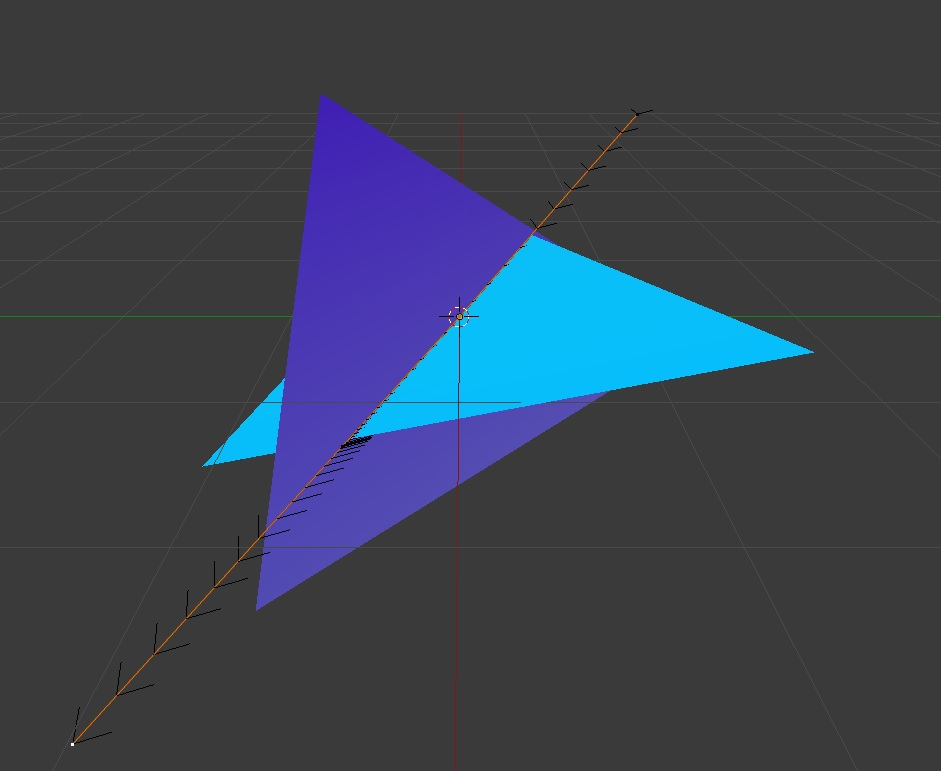
\includegraphics[width=220pt]{imgs/AsseMozzi.jpg}
		\caption{Calcolo dell'asse del Mozzi attraverso intersezione dei piani omologhi}
		\label{rot:gb:imgMozzi}
	\end{figure} 
\end{frame}

\begin{frame}
\frametitle{Il metodo di Groebner: Il caso spaziale}
\begin{itemize}
	\item Siano $\hat{j_1}, \hat{j_1}^{'} \in \mathbb{R}^2$ i versori della proiezione di una qualsiasi coppia omologa sul piano passante per l'origine e ortogonale all'asse del Mozzi. Si può calcolare l'angolo compreso tra i due versori:
	\begin{equation}
	\theta_1 = arcos(\frac{\hat{j_1} \cdot \hat{j_1}^{'}}{\| \hat{j_1}\| \|\hat{j_1}^{'}\|})
	\end{equation}
	Si sceglie la soluzione che permette di ottenere una rotazione propria al passo successivo.
	\item Si può definire la prima rotazione, utilizzando la rappresentazione asse-angolo come:
	\begin{equation}
	R_1 = Rot(asse_{mozzi}, \theta_1)
	\end{equation} 
\end{itemize}
\end{frame}

\begin{frame}
\frametitle{Il metodo di Groebner: Il caso spaziale}

\begin{figure}[h]
	\centering
	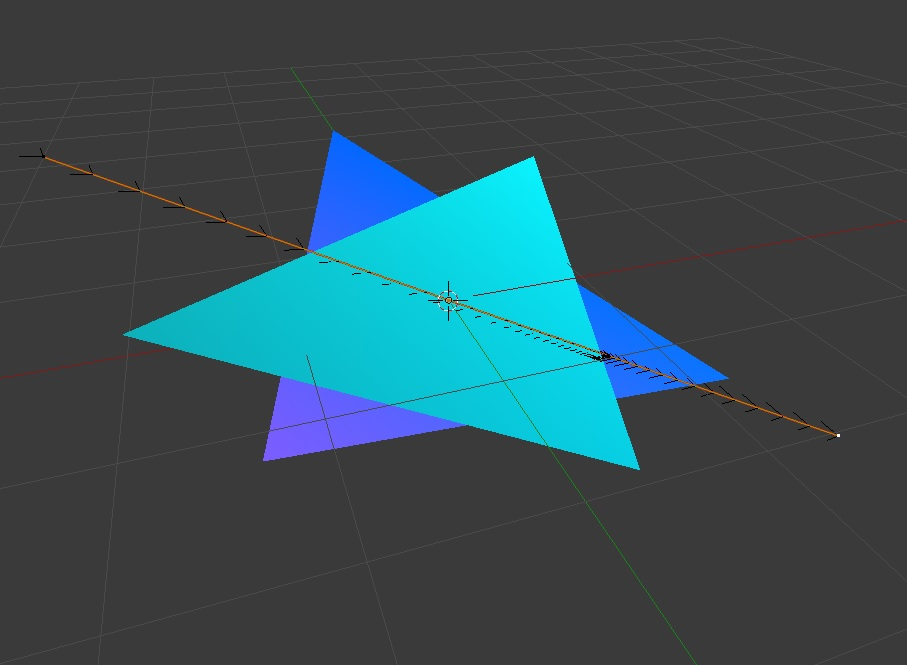
\includegraphics[width=240pt]{imgs/PianiSuStessoPiano.jpg}
	\caption{Dopo la rotazione sull'asse del Mozzi i due piani sono equi orientati}
	\label{rot:gb:samePlane}
\end{figure} 
\end{frame}

\begin{frame}
\frametitle{Il metodo di Groebner: Il caso spaziale}
\begin{itemize}
	\item Si può utilizzare quanto fatto nel planare:
	\begin{center}
		$cos(\theta_2) = \phi_4(R_1p_1, p_1^{'}, R_1p_2, p_2^{'})/\phi_d(R_1p_1, p_1^{'}, R_1p_2, p_2^{'}), \,\,$\\
		$sin(\theta_2) = \phi_3(R_1p_1, p_1^{'}, R_1p_2, p_2^{'})/\phi_d(R_1p_1, p_1^{'}, R_1p_2, p_2^{'}),$
	\end{center} 
	Si calcola l'angolo
	\begin{equation}
	\theta_2 = atan_2(cos(\theta_2), sin(\theta_2))
	\end{equation} 
	\item Si può definire la seconda rotazione, utilizzando la rappresentazione asse-angolo, come la rotazione intorno ad un asse unitario passante per l'origine e ortogonale ai piani.
	\begin{equation}
	R_2 = Rot(asse_{\bot Piano}, \theta_2)
	\end{equation} 
\end{itemize}
\end{frame}

\begin{frame}
\frametitle{Il metodo di Groebner: Il caso spaziale}
\begin{itemize}
	\item Si ottiene la matrice di rotazione risultant pre-moltiplicando $R_1$ per $R_2$, perché trasformazioni applicate in sequenza nel riferimento mobile solidale al primo piano.
	\begin{equation}
	R = R_2R_1, R \in \mathbb{R}^{3 \times 3}
	\end{equation}
	\item Il vettore di traslazione può essere calcolato confrontando i centroidi al netto della rotazione:
	\begin{equation}
	t = w_c^{'} - Rw_c, t \in \mathbb{R}^3
	\end{equation}
	\item la matrice di trasformazione può essere calcolata come una roto-traslazione.
\end{itemize}
\end{frame}

\subsection{Il metodo di Kabsch}
%\begin{frame}
%\frametitle{Il metodo di Kabsch}
%kabsch
%\Huge{\centerline{Il metodo di Kabsch}}
%\end{frame}

\begin{frame}
\frametitle{Il metodo di Kabsch}
%kabsch
\begin{block}{Kabsch's Algoritmh}
	\begin{itemize}
		\item presentato per la prima volta nel 1974 ad opera di W. Kabsch
		\item algoritmo di tipo: adattativo
		\item utilizzo tipico: bio-informatica confronto tra proteine	
	\end{itemize}
\end{block}
\end{frame}

\begin{frame}
\frametitle{Il metodo di Kabsch}
%kabsch
\begin{itemize}
	\item Siano dati due set di punti omologhi $a_1, \dots, a_N$ e $b_1, \dots, b_N$
	\item Si procede traslando i set di punti facendo si che i centroidi coincidano con l'origine:
	\begin{equation}
	\label{rot:eq:redef}
	x_i = a_i - a_c, \, \, 
	y_i = b_i - b_c
	\end{equation}
	\item Si fissa quindi l'indice di costo $J = d(x, y)$
	\begin{equation}
	\label{rot:eq:dist}
	d(x, y) =  \frac{1}{N}\sum_{i = 1}^{N} \| R x_i - y_i \|^2
	\end{equation}	
\end{itemize}
\end{frame}

\begin{frame}
\frametitle{Il metodo di Kabsch}
%kabsch
\begin{itemize}
	\item Si possono rappresentare i set di punti attraverso le matrici:
	\begin{equation}
	X = [x_1 \, x_2 \, ... \, x_N], Y = [y_1 \, y_2 \, ... \, y_N], X, Y \in \mathbb{R}^{d \times N},
	\end{equation}
	e sia $X^{'} = RX, \, \, X^{'} = [x_1^{'} \, x_2^{'} \, ... \, x_N^{'}]$ la matrice dei punti ruotati.
	\item Possiamo allora scrivere che:
	\begin{equation}
	N J = \sum_{i = 1}^{N} \| x_i^{'} - y_i \|^2 = Tr[(X^{'} - Y)^{T}(X^{'} - Y)]
	\end{equation}
\end{itemize}
\end{frame}

\begin{frame}
\frametitle{Il metodo di Kabsch}
%kabsch
\begin{itemize}
	\item Grazie alla linearità dell'operatore traccia vale che:
	\begin{equation}
	Tr[(X^{'} - Y)^{T}(X^{'} - Y)] = Tr(X^{'T}X^{'}) + Tr(Y^{T}Y) - 2Tr(Y^{T}X^{'})
	\end{equation}
	\item Inoltre vale l'identità:
	\begin{equation}
	\label{rot:eq:mod}
	Tr(X^{'T}X^{'}) + Tr(Y^{T}Y) = \frac{1}{N}\sum_{i = 1}^{N} \| x_i^{'} \| ^ 2 + \| y_i \| ^ 2
	\end{equation}
	che grazie alla traslazione dei centroidi sull'origine è costante e può essere eliminata dall'indice di costo.
\end{itemize}
\end{frame}

\begin{frame}
\frametitle{Il metodo di Kabsch}
%kabsch
\begin{itemize}
	\item Per risolvere il problema allora basterà massimizzare la quantità
	\begin{equation}
		Tr(Y^{T}X^{'}) = Tr(Y^{T}RX) = Tr((XY^{T})R)
	\end{equation}
	\item La matrice $ C = XY^{T}, \, C \in \mathbb{R}^{d \times d}$ è la matrice di cross correlazione tra i due set.
	\item Si usa ora la decomposizione SVD della matrice $C = VSW^T$, si ha che $V, S, W^T \in \mathbb{R}^{d \times d}$ poiché $C$ è quadrata. La matrice $S$ è diagonale e i suoi elementi sono i valori singolari della matrice $C$ in ordine decrescente.
\end{itemize}
\end{frame}

\begin{frame}
\frametitle{Il metodo di Kabsch}
%kabsch
\begin{itemize}
	\item Dato che per l'operatore traccia vale che $Tr(AB) = Tr(BA)$, indicando con $A = V$ e $B = SW^TR$ è possibile scrivere:
	\begin{equation}
	Tr(Y^{T}X^{'}) = Tr(VSW^TR) = Tr(SW^TRV) = \sum_{i = 1}^{d} s_iw_i^TRv_i
	\end{equation}
	\item La matrice $T = W^TRV$ è ortonormale, questo vuol dire che i suoi elementi non potranno avere modulo maggiore di 1. Pertanto indicando con $T_{ii} = w_i^TRv_i$ gli elementi sulla diagonale di $T$, vale che
	\begin{equation}
	Tr(Y^{T}X^{'}) = \sum_{i = 1}^{d} s_iT_{ii} \leq \sum_{i = 1}^{d} s_i
	\end{equation}
	pertanto al massimo il valore della quantità $Tr(Y^{T}X^{'})$ è pari alla somma dei valori singolari $s_i$.
\end{itemize}
\end{frame}

\begin{frame}
\frametitle{Il metodo di Kabsch}
%kabsch
\begin{itemize}
	\item Si deve fare in modo quindi che la matrice $T$ sia una matrice identità.
	Grazie alla proprietà di $V$ e $W^T$ di essere ortonormali, $VV^T = I, W^TW = I$, basterà scegliere:
	\begin{equation}
	R = WV^T
	\end{equation}
	\item Resta da risolvere un problema, cioè che in generale $det(R) = \pm 1$, il caso negativo va evitato.
	Per fare ciò possiamo aggiungere il vincolo che $det(R) = 1$.
\end{itemize}
\end{frame}

\begin{frame}
\frametitle{Il metodo di Kabsch}
%kabsch
\begin{itemize}
	\item  Notando che $s_1 \ge s_2 \ge \, ... \, \ge s_d$ e che
	\begin{equation}
	Tr(Y^{T}X^{'}) = \sum_{i = 1}^{d} s_iT_{ii} 
	\end{equation}
	possiamo individuare il massimo per questa quantità, rispettando il vincolo, con la scelta $T_{11} = T_{22} = \, ... \, = T_{d-1d-1} = 1, T_{dd} = -1$.
	\item Infatti, grazie alla richiesta di ortonormalità, deve valere che i $T_{ii} = \pm 1$.
\end{itemize}
\end{frame}

\begin{frame}
\frametitle{Il metodo di Kabsch}
%kabsch
\begin{itemize}
	\item La soluzione si ottiene pertanto come:
	\begin{equation}
	R = W
	\begin{bmatrix}
	1 \,\, 0 \,\, \cdots \,\, 0\\
	0 \,\, 1 \,\, \cdots \,\, 0\\
	\vdots\\
	0 \,\, \cdots \,\, 1 \,\, 0\\
	0 \,\, \cdots \,\, 0 \,\, d\\
	\end{bmatrix}V^T
	,\; \; \; \; 
	d = sign(det(WV^T))
	\end{equation}
	
	\item Analogamente al caso precedente, 
	\begin{equation}
	t = b_c - Ra_c, t \in \mathbb{R}^d
	\end{equation}
	dove $b_c$ e $a_c$ sono i centroidi precedentemente calcolati.
\end{itemize}
\end{frame}

\begin{frame}
\frametitle{Il metodo di Kabsch: robustezza ai disturbi}
%kabsch
\begin{itemize}
	\item Considerando $\tilde{x_i}$ la i-esima misura disturbata, si ha che
	\begin{equation}
	x_c = \frac{1}{N}\sum_{i = 1}^{N} \tilde{x_i} = \frac{1}{N}\sum_{i = 1}^{N} x_i + e_i \longrightarrow \hat{x} + E[e] = \hat{x}
	\end{equation}
	\begin{equation}
	c_{ij} = \sum_{k = 1}^{N}  \tilde{X_{ik}} \tilde{Y_{kj}} \longrightarrow \sum_{k = 1}^{N} X_{ik} Y_{kj} + (\cdots) \begin{bmatrix}
	E[e_x] \\
	E[e_y]
	\end{bmatrix} = \hat{c_{ij}}
	\end{equation}
	dove con $E[e]$ si indica il valore atteso del disturbo, supposto rumore bianco.
	\item Al crescere del numero di campioni i centroidi e la matrice di cross-correlazione calcolati tendono a quelli "veri". Il risultato stimato dall'algoritmo tende a quello vero.
\end{itemize}
\end{frame}

%------------------------------------------------
\section{Visione artificiale}
%\begin{frame}
%\frametitle{Visione artificiale}
%kabsch
%\Huge{\centerline{Visione artificiale}}
%\end{frame}

\begin{frame}
\frametitle{Visione artificiale}
%problema generazione punti
\begin{block}{Problema}
	è possibile calcolare/misurare le coordinate, nel sistema di riferimento solidale all'osservatore mobile, di un insieme di punti omologhi appartenenti al mondo circostante? 
	Il mondo circostante si suppone ignoto.  
\end{block}

\textbf{Soluzione}: 
\begin{itemize}
	\item Feature detection:  FAST + BRIEF + BF matcher
	\item Stereovisione
\end{itemize}
\end{frame}

\subsection{Features detection}
\begin{frame}
\frametitle{Features detection: che cos'è una feature?}
%feature 

\begin{figure}[h]
	\centering
	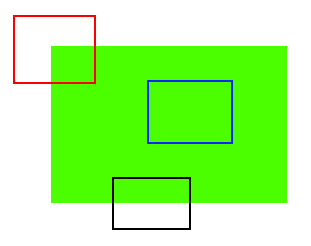
\includegraphics[width=200pt]{imgs/feature_simple.png}
	\caption{Individuazione delle Features.}
	\label{vis:feature:detect}
\end{figure} 
\end{frame}

\begin{frame}
\frametitle{Features detection: FAST}
%fast
\begin{itemize}
	\item L'algoritmo FAST (Feature from Accelerated Segment Test) è adibito all'estrazione dei punti chiave.
	\item Caratteristiche: molto efficace, veloce e parallelizzabile.
	\item Funzionamento: pre-test veloce, segment test, non-maximus suppression.
\end{itemize}
\begin{figure}[h]
	\centering
	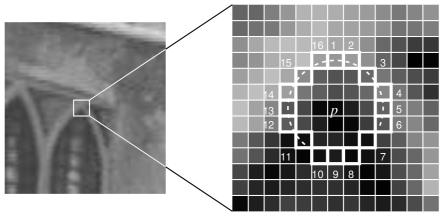
\includegraphics[width=200pt]{imgs/fast_speedtest.jpg}
	\caption{Fast Segment test.}
	\label{vis:feature:Fast}
\end{figure}
\end{frame}

\begin{frame}
\frametitle{Features detection: FAST}
%fast
\begin{figure}[h]
	\centering
	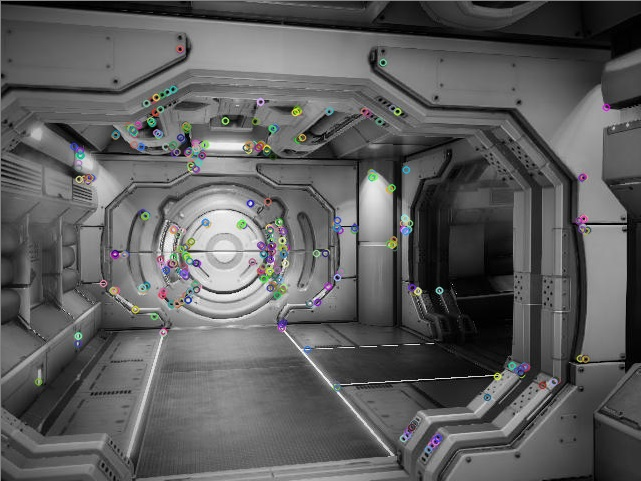
\includegraphics[width=200pt]{imgs/fdetection.jpg}
	\caption{Risultato dell'esecuzione dell'algoritmo FAST.}
	\label{vis:feature:detection}
\end{figure}
\end{frame}

\begin{frame}
\frametitle{Features description: BRIEF}
%brief
\begin{itemize}
	\item L'algoritmo BRIEF, Binary Robust Independent Elementary Features, genera dei descrittori sotto forma di stringhe di bit. 
	\item Il confronto tra due keypoint può essere fatto in modo estremamente efficiente, con una sola operazione XOR.
	\item pattern di confronto: uniforme, normale, randomico. 
	\item Per ogni bit della stringa ed in base al pattern scelto se ne fissa il valore secondo la formula:
	\begin{equation}
	\tau_i(p, q_i) := \begin{cases}
	1, \qquad se \; I_p \leq I_{q_i}\\
	0, \qquad altrimenti
	\end{cases}
	\end{equation}
	dove con $p$ si è indicato il pixel punto chiave, $q_i$ l'i-esimo pixel scelto in base al pattern.
\end{itemize}
\end{frame}

\begin{frame}
\frametitle{Features matching: Forza bruta}
%bf
\begin{itemize}
	\item I confronti vengono effettuati su base dei descrittori con algoritmo a forza bruta.
	\item Vantaggio: facilmente parallelizzabile.
\end{itemize}
\begin{figure}[h!]
	\centering
	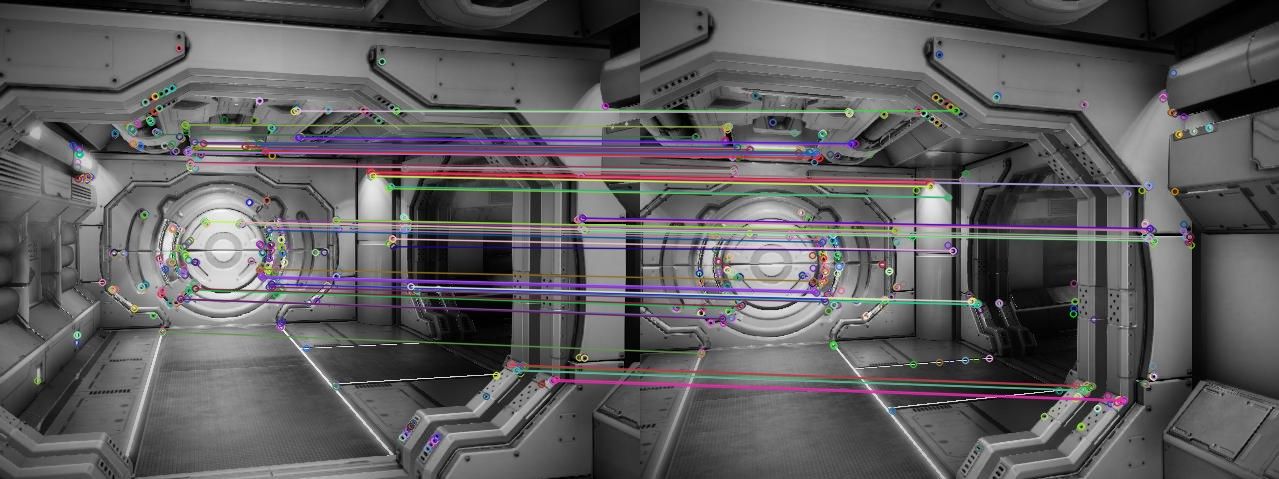
\includegraphics[width=250pt]{imgs/TwoInstantDetection.jpg}
	\caption{Risultato dell'esecuzione del comparatore: FAST + BRIEF + Brute Force matcher su due immagini in due punti di osservazione diversi}
	\label{vis:feature:risTwo}
\end{figure}
\end{frame}

\subsection{Stereovisione: calcolo delle coordinate 3D}

\begin{frame}
\frametitle{Il sensore fotografico}
%stereo
Un sensore fotografico può essere modellato come nella seguente figura. Tale modello è detto \textbf{Pinhole camera}.
\begin{itemize}
	\item Un singolo raggio di luce, da ogni angolazione, supera il pinhole e si infrange sul piano di cattura o film.
\end{itemize}
\begin{figure}[h!]
	\centering
	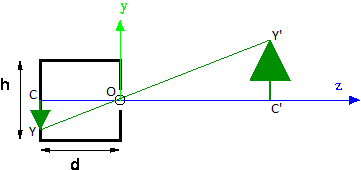
\includegraphics[width=150pt]{imgs/pinhole-and-tree2.png}
	%\caption{Esempio cattura immagine con sensore pinhole.}
	\label{vis:stereo:pinhole}
\end{figure} 
\end{frame}

\begin{frame}
\frametitle{Il sensore fotografico}
%stereo
Modello \textbf{Pinhole camera sintetico}.
\begin{itemize}
	\item Il piano di cattura viene capovolto.
\end{itemize}
\begin{figure}[h!]
	\centering
	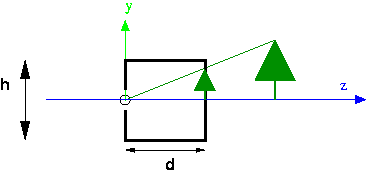
\includegraphics[width=150pt]{imgs/synthetic-and-tree.png}
	\caption{Esempio cattura immagine con sensore sintetico.}
	\label{vis:stereo:virtuale}
\end{figure} 
\end{frame}

\begin{frame}
\frametitle{Stereovisione}
%stereo
\begin{itemize}
	\item Almeno due sensori sono necessari per la ricostruzione dell'informazione tridimensionale.
\end{itemize}
\begin{figure}[h!]
	\centering
	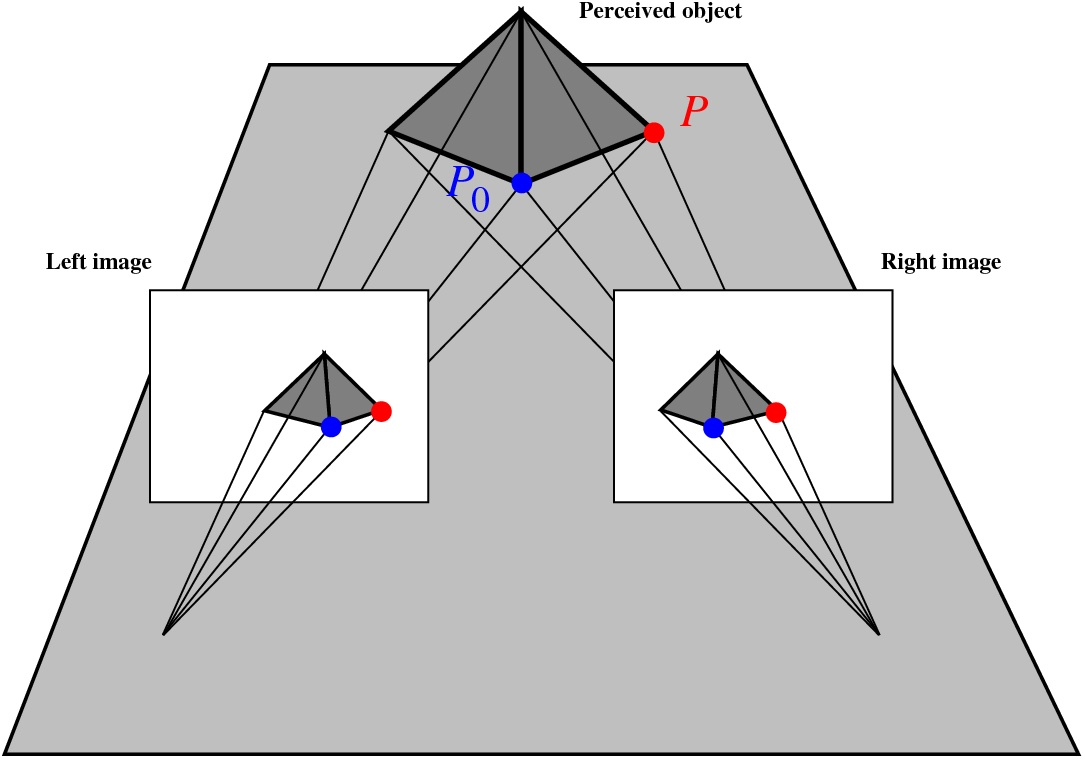
\includegraphics[width=200pt]{imgs/stereo2.jpg}
	\caption{Coppia di immagini catturate da due sensori differenti nella scena.}
	\label{vis:stereo:pair}
\end{figure} 
\end{frame}

\begin{frame}
\frametitle{Stereovisione: centro di fissazione all'infinito}
\begin{itemize}
	\item Il calcolo può essere effettuato ragionando per triangoli simili.
\end{itemize}
\begin{figure}[h!]
	\centering
	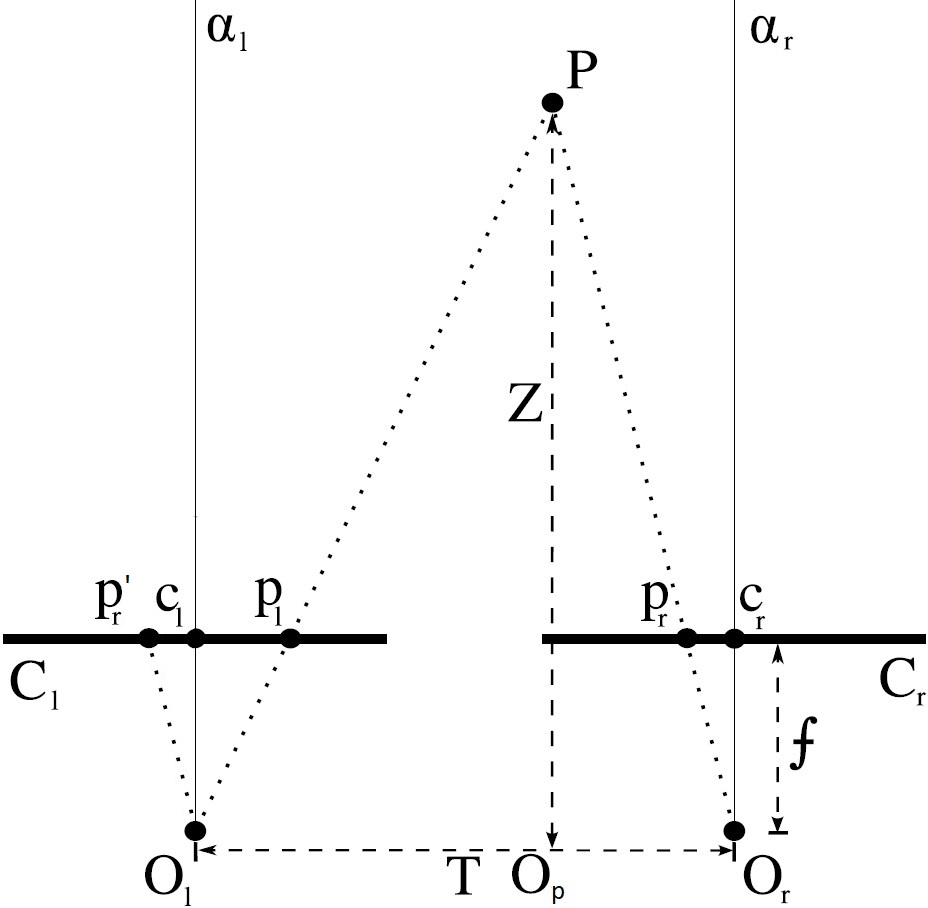
\includegraphics[width=150pt]{imgs/stereo.jpg}
	\caption{Configurazione sistema stereoscopico.}
	\label{vis:stereo:sistem}
\end{figure}
\end{frame}

\begin{frame}
\frametitle{Stereovisione: soluzione}
\begin{itemize}
	\item Si estrae per ciascun punto dalla coppia di immagini l'informazione di disparità, cioè la differenza in pixel della rispettiva coordinata X.
	\begin{equation}
		d := p_{l_x} - p_{r_x}, d \ge 0, d \in \mathbb{Z}
	\end{equation}
	\item Le coordinate di ciascun punto si calcolano nella seguente maniera:
	\begin{align}
	X &:= \frac{(p_{l_x} - c_{l_x}) T}{d},\\
	Y &:= \frac{(p_{l_y} - c_{l_y}) T}{d},\\
	Z &:= \frac{Tf}{d}
	\end{align}
\end{itemize}
\end{frame}

\begin{frame}
\frametitle{Stereovisione: calcolo disparità}
\begin{itemize}
	\item Si può utilizzare ancora il features detection per individuare lo stesso punto nella coppia di foto stereo e calcolarne la disparità.
\end{itemize}
\begin{figure}[h!]
	\centering
	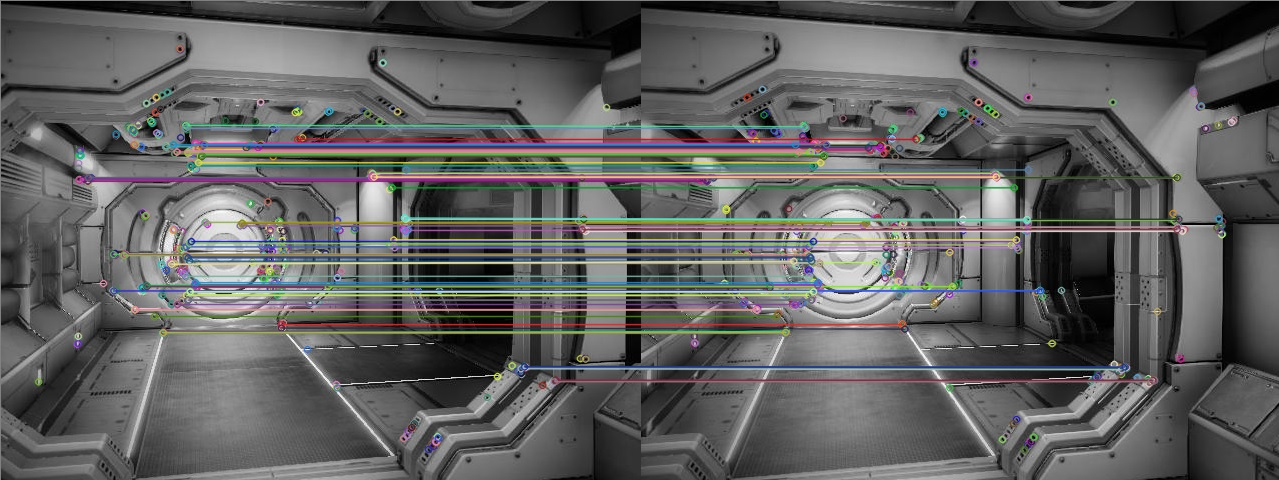
\includegraphics[width=300pt]{imgs/stereoDetection.jpg}
	\caption{Risultato dell'esecuzione del comparatore: FAST + BRIEF + Brute Force matcher su una coppia di immagini stereo.}
	\label{vis:feature:risStereo}
\end{figure} 
\end{frame}

%------------------------------------------------
\section{Implementazione}

\subsection{Analisi dei requisiti}
\begin{frame}
\frametitle{Analisi dei requisiti}
%tool
\begin{itemize}
	\item \textbf{Piattaforma:}  fissa e mobile,
	\item \textbf{Architettura target:}  x86\_64, ARM,
	\item \textbf{Sistema Operativo target:}  Windows, GNU/Linux,
	\item \textbf{Specifiche hardware minime:}
	\begin{itemize}
		\item CPU: x86\_64 o ARM,
		\item GPU: nessuna o generica con supporto OpenCL,
	\end{itemize} 
	\item \textbf{Specifiche hardware consigliate:}
	\begin{itemize}
		\item CPU: x86\_64 o ARM con supporto OpenCL o SIMD/AVX,
		\item GPU: coprocessore grafico Nvidia ad alte prestazioni con supporto CUDA Shared Model $\ge$ 2.1,
	\end{itemize}
	\item \textbf{Linguaggio di sviluppo:} C++, OpenCV	
	\item \textbf{Implementazioni:} CPU/SIMD, OpenCL, CUDA	 
\end{itemize}
\end{frame}

\subsection{L'architettura}
\begin{frame}
\frametitle{L'architettura}
%arch
\begin{figure}[h!]
\centering
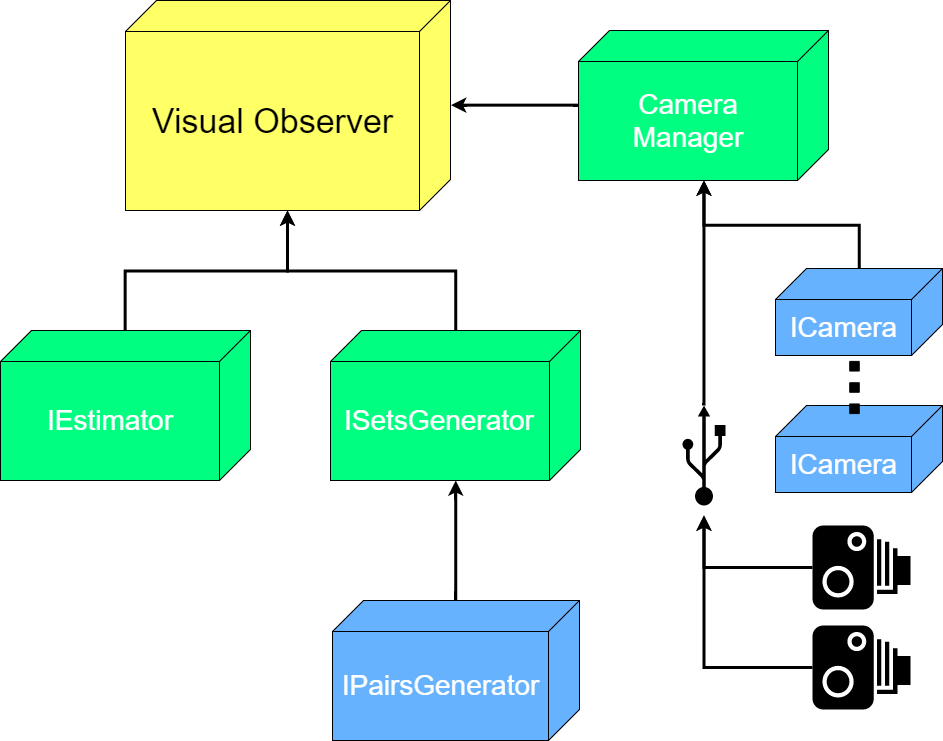
\includegraphics[width=200pt]{imgs/arch.png}
\caption{Rappresentazione architettura software Visual Observer.}
\label{vis:impl:arch}
\end{figure} 
\end{frame}


%-------------------------------------------------
\section{Test delle prestazioni}
\begin{frame}
\frametitle{Ambiente virtuale}
%arch
\begin{figure}[h!]
	\centering
	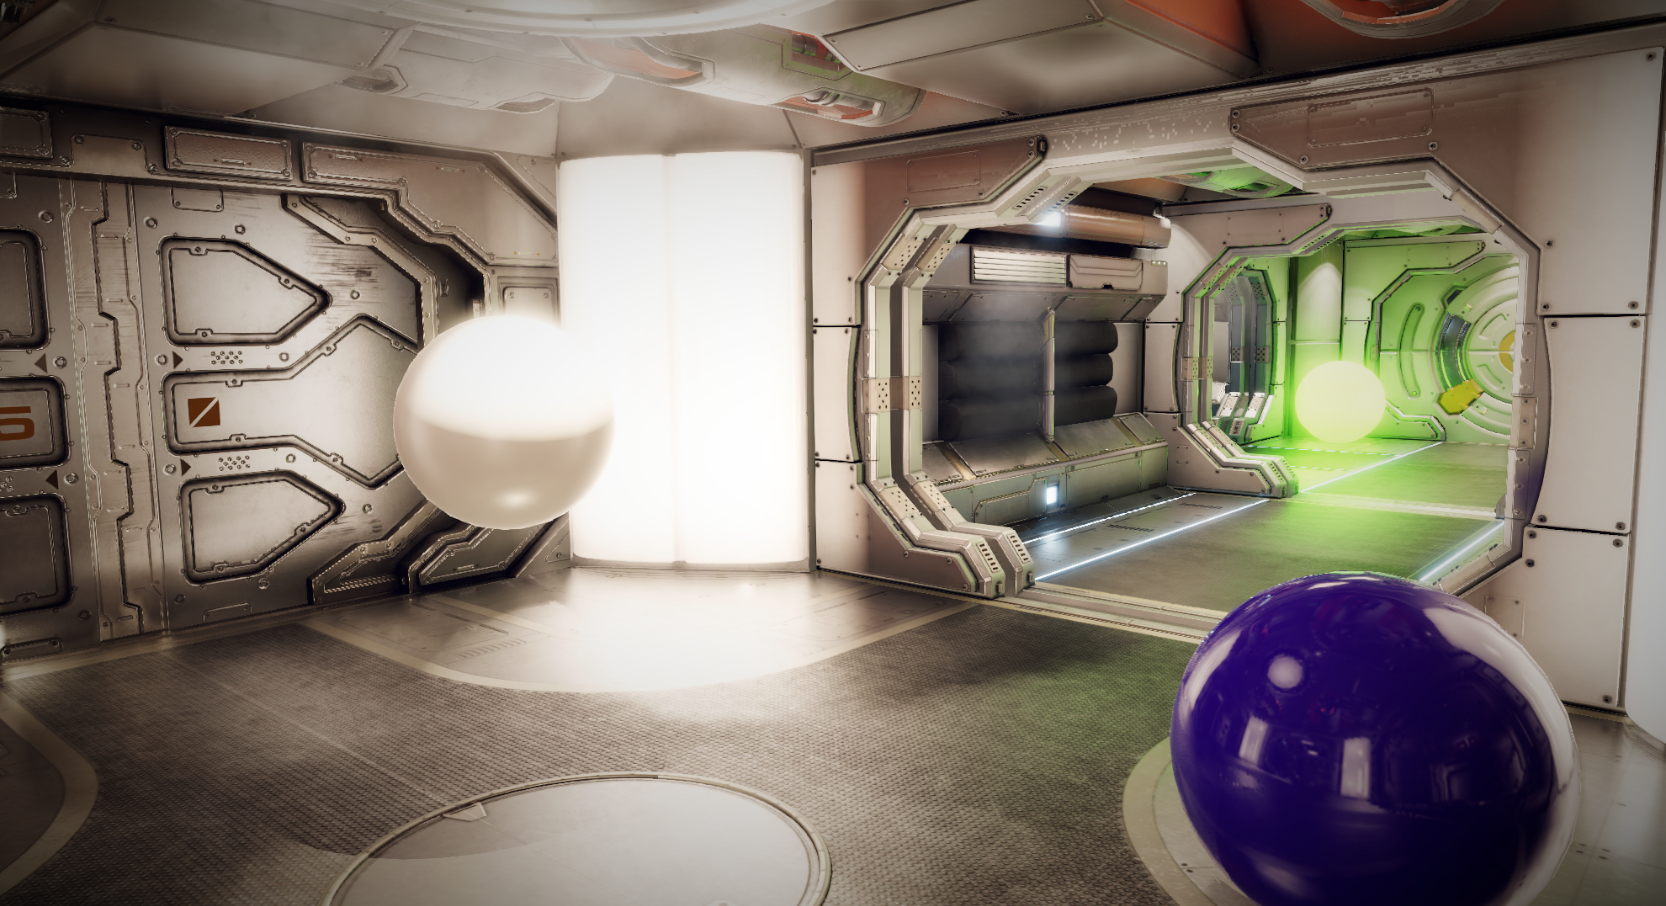
\includegraphics[width=320pt]{imgs/zona2.png}
	\caption{Ambiente virtuale generato con motore grafico Unity3D.}
	\label{vis:virtual}
\end{figure} 
\end{frame}

\begin{frame}
\frametitle{Test effettuati}
%arch
I test sono stati effettuati sulla seguente macchina:
\begin{itemize}
	\item \textbf{CPU:} Intel i7-6700HQ @ 2.60 GHz,
	\begin{itemize}
		\item \textbf{Architettura:} x86\_64, 
		\item \textbf{Specifiche:} AVX, AVX2, OpenCL,
	\end{itemize}		
	\item \textbf{Memoria:} 16 GB, 
	\item \textbf{GPU:} Nvidia Geforce GTX 1070,
	\begin{itemize}
		\item \textbf{Memoria dedicata:} 8 GB, 
		\item \textbf{Specifiche:} OpenCL, CUDA SM 6.1
	\end{itemize}			
	\item \textbf{Sistema Operativo:}  Windows.	 
\end{itemize}
\end{frame}

\begin{frame}
\frametitle{Test effettuati}
%arch
\begin{itemize}
	\item \textbf{Algoritmi di stima:}
	\begin{itemize}
		\item \textbf{Errore in misura} N(0, $10^{-3} \div 10^{-1}$)
		\item \textbf{Groebner:}
			\begin{itemize}
				\item \textbf{Tempo esecuzione:} $10^{-6}$ sec
				\item \textbf{Errore di stima:} \hspace{10pt} $10^{-3} \div 10^{-1}$ (errore quadratico sulle matrici)
			\end{itemize} 
		\item \textbf{Kabsch:}
		\begin{itemize}
			\item \textbf{Numero punti:} \hspace{28pt} $3 \div 10^{4}$ 
			\item \textbf{Tempo esecuzione:} $10^{-6} \div 10^{-5}$ sec
			\item \textbf{Errore di stima:} \hspace{10pt} $10^{-3} \div 10^{-5}$ (errore quadratico sulle matrici)
		\end{itemize} 
	\end{itemize}		
	\item \textbf{Visual observer:}
	\begin{itemize}
		\item \textbf{Risoluzione immagini:} 640x480 pixels
		\item \textbf{Max KeyPoint:} 500
		\item \textbf{Tempo esecuzione:}
		\begin{itemize}
			\item \textbf{CPU:}  \hspace{11pt}  0.450 sec
			\item \textbf{OpenCL:} 0.027 sec
			\item \textbf{CUDA:} \hspace{4pt} 0.031 sec
		\end{itemize}
		\item \textbf{Errore di stima:} $\approx 10^{-2}$ unità Unity
	\end{itemize} 		
	
\end{itemize}
\end{frame}

%------------------------------------------------
\section{Conclusioni e sviluppi futuri}

\begin{frame}
\frametitle{Conclusioni}
%conl
\begin{itemize}
	\item Si sono studiati nuovi strumenti innovativi:
	\begin{itemize}
		\item geometria algebrica
		\item stereovisione
	\end{itemize}
	\item Si è progettato e implementato un software di stima della posizione ed orientamento basato su tali strumenti
	\item Si è utilizzato un motore grafico per generare un mondo virtuale di test.
	\item Si sono valutate le performance ottenute, soprattutto in ottica di una futura implementazione real-time
\end{itemize}
\end{frame}

\begin{frame}
\frametitle{Sviluppi futuri}
%conl
\begin{itemize}
	\item Prevedere la possibilità di gestire diversi oggetti dinamici.
	\begin{itemize}
		\item a livello di stima: multy body Procustes
		\item a livello di identificazione: machine learning per riconoscimento degli oggetti mobili.
	\end{itemize}
	\item Costruire un prototipo e sperimentarne il funzionamento in un contesto reale.
	\item Migliorare l'integrazione con Unity: input online, controllo agente.
	\item Bug-fix, varie ed eventuali.
\end{itemize}
\end{frame}

%------------------------------------------------
\begin{frame}
\frametitle{Grazie}
%conl
\Huge{\centerline{Grazie per l'attenzione!}}
\end{frame}

\end{document} 